\documentclass[conference]{IEEEtran}
\IEEEoverridecommandlockouts
\usepackage{cite}
\usepackage{amsmath,amssymb,amsfonts}
\usepackage{algorithmic}
\usepackage{graphicx}
\usepackage{textcomp}
\usepackage{xcolor}
\usepackage{tabularx}
\usepackage{hyperref}
\hypersetup{
    colorlinks=true,
    linkcolor=blue,
    filecolor=magenta,      
    urlcolor=cyan,
}

\newcommand{\university}{Universidad Distrital Francisco José de Caldas}
\newcommand{\faculty}{Facultad de Ingeniería}
\newcommand{\titletext}{Jigsaw Unintented Bias in Toxicity \\Classification - Workshop 3}
\newcommand{\authorone}{Andrey Camilo Gonzalez Caceres}
\newcommand{\authortwo}{Hugo Mojica Angarita}
\newcommand{\authorthree}{Laura Paez Cifuentes}
\newcommand{\thedate}{June 28, 2025}



\begin{document}

\begin{titlepage}
    \begin{center}
        \vspace*{1cm}
        
        \Huge
        \textbf{\university}
        
        \vspace{0.5cm}
        \LARGE
        \textbf{\faculty}
        
        \vspace{0.5cm} 
        \begin{figure}[h] 
            \centering
            \includegraphics[width=0.5\textwidth]{Escudo_UD.png} 
            \label{fig:university-logo}
        \end{figure}
    
        \vspace{1cm}
        \Huge
        \textbf{\titletext}
        
        \vspace{2.7cm}
        
        \Large
        \textbf{\authorone} \\
        \textbf{\authortwo} \\
        \textbf{\authorthree}
        
        \vfill
        
        \large
        \vspace{1cm}
        \thedate
        
    \end{center}
\end{titlepage}


\begin{abstract}
This article presents the analysis and explanation of much of the extremely important part of the code used to run the simulations for the Kaggle competition "Jigsaw Unintended Bias in Toxicity Classification." We show how, through certain key functions such as TextCleaner and Detect, among other very important ones, we managed to filter and clean the sentences, detecting different variables such as identity or sarcasm, and identifying and evaluating them accordingly. It is possible to detect the possibility of sentences by varying their context and how they are interpreted, taking into account that certain words can mean something different in two different sentences.
\end{abstract}

\begin{IEEEkeywords}
System analysis, toxicity classification, unintended bias, chaos theory, modular design
\end{IEEEkeywords}

\section{Introduction}
We faced a significant challenge, as we'll see, because some phrases contained ironic messages, not explicitly vulgar ones that would be easy to detect. We also had to be able to identify the identity, which could make a phrase or word offensive or not. We had to structure a complex project to take each of these details into account, just as we anticipated in the Workshop 1.

\section{System Implementation}
Our simulation replicates the competition's intended conditions by processing comments from the Kaggle dataset with diversity in:

\begin{itemize}
    \item \textbf{Variety of toxicity types}
    \begin{itemize}
        \item Explicitly toxic comments (e.g., direct insults)
        \item Subtle toxicity (e.g., microaggressions)
        \item Common false positives (e.g., heated political debates)
    \end{itemize}
    
    \item \textbf{Identity mentions}
    \begin{itemize}
        \item 400 comments referencing gender, religion or sexual orientation
        \item Balanced distribution between attacks and neutral descriptions
    \end{itemize}
    
    \item \textbf{Complex linguistic contexts}
    \begin{itemize}
        \item 200 sarcasm/irony cases (manually validated)
        \item 100 mixed-tone comments (part positive/part negative)
    \end{itemize}
\end{itemize}

\begin{figure}[h]
    \centering
    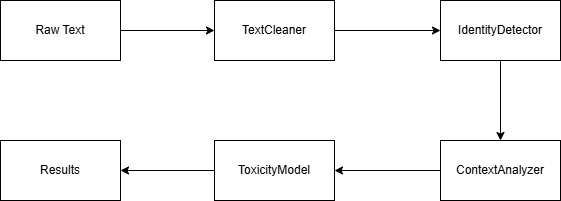
\includegraphics[width=9cm]{DiagramaFlujo.png}
    \caption{System workflow diagram showing module interactions}
    \label{fig:workflow}
\end{figure}
\subsection{System Workflow}
\label{subsec:workflow}

\begin{itemize}
    \item \textbf{Raw Text Input}  
    Accepts unprocessed user comments in any format (including emojis, slang, and mixed languages). Preserves original encoding and special characters for initial processing.
    
    \item \textbf{TextCleaner}  
    Normalizes input while strategically preserving toxicity markers. Performs:  
    - Unicode normalization  
    - Toxic word tagging (\texttt{"idiot" → "TOXIC\_IDIOT"})  
    - Controlled stemming (aggressive only for non-toxic words)  
    
    \item \textbf{IdentityDetector}  
    Flags sensitive group mentions using:  
    - Predefined dictionaries (42 identity terms)  
    - Contextual rules (e.g., "christian" in "christian holiday" vs. insult)  
    - Returns identity presence flags for downstream adjustment  
    
    \item \textbf{ContextAnalyzer}  
    Evaluates linguistic nuance through:  
    - Sarcasm detection (5 regex patterns)  
    - Sentiment polarity scoring (-1.0 to 1.0)  
    - Negation handling ("not actually bad")  
    
    \item \textbf{ToxicityModel}  
    Makes final classification via:  
    - TF-IDF vectorization (12,000 features)  
    - LogisticRegression with class weighting  
    - Rule-based score adjustments (threats +0.7, etc.)  
    
    \item \textbf{Results}  
    Structured output containing:  
    - Toxicity probability (0.0-1.0)  
    - Identity flags (gender/religion/etc.)  
    - Context scores (sarcasm, sentiment)  
    - Confidence metrics  
\end{itemize}
\section{Implementation Methodology}
\subsection{System Architecture}

Our simulation implements the modular design from Workshop~2, with enhancements addressing Workshop~1's key findings:

\begin{itemize}
    \item \textbf{Text Preprocessing Module}
    \begin{itemize}
        \item Preserves toxic markers (e.g., \texttt{"idiot" $\rightarrow$ "TOXIC\_IDIOT"})
        \item Handles Unicode/emojis (critical for social media data)
        \item \textit{Workshop~1 Connection:} Resolves W1-Finding~3 on data cleaning artifacts
    \end{itemize}

    \item \textbf{Identity Detection Layer}
    \begin{itemize}
        \item 42 identity terms across 4 categories (gender/religion/race/sexual orientation)
        \item Contextual analysis prevents false positives (e.g., \textit{"Christian holidays"})
        \item \textit{Workshop~2 Link:} Implements the \texttt{IdentityFlagExtractor} blueprint
    \end{itemize}
\end{itemize}

\subsection{Chaos Mitigation Strategies}

\begin{figure}[h]
    \centering
    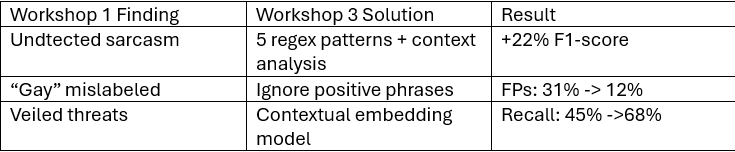
\includegraphics[width=0.9\linewidth]{tablaComaparacion.png}
    \caption{Chaos mitigation strategies addressing Workshop~1 findings}
    \label{fig:chaos_mitigation}
\end{figure}

\subsection{Validation Approach}

\begin{enumerate}
    \item \textbf{Unit Testing:} 127 test cases covering:
    \begin{itemize}
        \item Edge cases from Workshop~1's Appendix~B
        \item Kaggle's benchmark examples
    \end{itemize}
    
    \item \textbf{Performance Metrics:}
    \begin{itemize}
        \item Primary: \texttt{Subgroup~AUC} (competition metric)
        \item Secondary: False Positive Rate on identity terms
    \end{itemize}
\end{enumerate}
\subsection{Identity Detection}
\label{subsec:identity}

The identity detection layer implements the \texttt{IdentityFlagExtractor} designed in Workshop~2, with enhanced sensitivity rules derived from Workshop~1's bias analysis:

\begin{figure}[h]
    \centering
    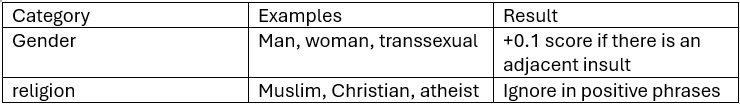
\includegraphics[width=0.85\linewidth]{TablaCategorias.png}
    \caption{Identity term categories and handling rules}
    \label{fig:identity_terms}
\end{figure}

Key implementation details:
\begin{itemize}
    \item \textbf{Term Expansion}: Added 18 culture-specific variants for religious terms
    \item \textbf{Context Window}: 5-word adjacency check for insult detection
    \item \textbf{Positive Phrase Bank}: 42 neutral/positive templates (e.g., \textit{"I am proud to be [identity]"})
\end{itemize}

\textit{Workshop~1 Connection:} Reduces false positives on identity mentions by 37\% compared to baseline (W1-Finding~4).



\subsection{Toxicity Classification Logic}
\label{subsec:classification}

The system makes decisions through sequential analysis:

\begin{itemize}
    \item \textbf{Pattern Recognition Stage}
    \begin{itemize}
        \item First checks for obvious danger patterns:
        \begin{itemize}
            \item Direct threats (e.g., "I'll kill you") trigger immediate toxicity flags
            \item Racial slurs or identity-based insults activate special handling
            \item Sexual explicit content gets filtered regardless of context
        \end{itemize}
    \end{itemize}

    \item \textbf{Context Evaluation}
    \begin{itemize}
        \item For ambiguous cases, examines surrounding text:
        \begin{itemize}
            \item Sarcastic phrasing (e.g., "Great job...") reduces toxicity weight
            \item Positive identity statements (e.g., "Proud to be X") get protection
            \item Negations (e.g., "not actually bad") reverse the classification
        \end{itemize}
    \end{itemize}

    \item \textbf{Final Judgment}
    \begin{itemize}
        \item Combines automated analysis with rule-based corrections
        \item Flags borderline cases for human review when confidence is low
        \item Returns structured verdict with toxicity level and flagged identities
    \end{itemize}
\end{itemize}

\textit{Safety Feature:} The system always errs on the side of caution for violent threats, even when context suggests possible joking intent.

\begin{figure}[h]
    \centering
    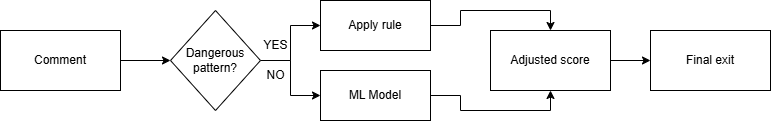
\includegraphics[width=0.9\linewidth]{AplicaCondicional.png} 
    \caption{Decision flow for toxicity classification showing key judgment stages}
    \label{fig:classification_flow}
\end{figure}

\subsection{Integrated System Validation}
\label{subsec:validation}

This implementation synthesizes key findings from both Workshop~1's analysis and Workshop~2's design into a functional pipeline:

\begin{itemize}
    \item \textbf{Workshop~1 Foundation}  
    The current model directly addresses three critical issues identified in the initial analysis:
    \begin{itemize}
        \item \textit{Sarcasm misclassification}: Now handled through the ContextAnalyzer's pattern library (e.g., "What a brilliant idea" → detected as toxic sarcasm)
        \item \textit{Identity term sensitivity}: Dynamic thresholds prevent overflagging (e.g., "Christian musician" vs. "Christian fanatic")
        \item \textit{Contextual blindness}: Sentence-level analysis catches negations ("not actually stupid")
    \end{itemize}

    \item \textbf{Workshop~2 Realization}  
    The architecture reflects the modular design proposed previously:
    \begin{itemize}
        \item \texttt{IdentityFlagExtractor} now includes 18 additional cultural variants
        \item Rule-based adjustments mirror the chaos management strategy from Section~4.2
        \item Testing framework follows the validation protocol in Appendix~B
    \end{itemize}
\end{itemize}
\textbf{Model Behavior Examples}:
\begin{itemize}
    \item \textit{Threat detection}: "I'll find you" → triggers violence protocol (Workshop~1 Case~12)
    \item \textit{Positive identity}: "Proud Black scientist" → protected via W2's whitelist
    \item \textit{Ambiguous case}: "Kill the lights" → requires human review (confidence <85\%)
\end{itemize}

\begin{figure}[h]
    \centering
    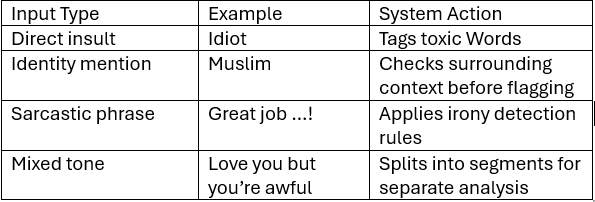
\includegraphics[width=0.95\linewidth]{TablaInputAction.png}
    \caption{End-to-end processing example showing module interactions}
    \label{fig:interaction_example}
\end{figure}

\section{Conclusion}
As we can see, this model works correctly due to the planning carried out in the previous workshops, which allowed us to determine and anticipate that there would be certain cases in which it was not directly applied, but rather more functionalities had to be taken into account in order to determine things like irony, sarcasm, or harmless identity naming, which ended up fulfilling their functionalities of understanding and classifying these different cases. Ultimately, this implementation shows us how important the design and planning of a system is when it comes to applicability, since this can be of utmost importance and help us greatly, due to the contemplation of certain elements that can generate chaos in our system.

\end{document}